\gil et \damien estimaient que le projet et les besoins du client collaient plus à la réalisation de plusieurs sous projets. Le projet \og bouclage de production \fg a ainsi été en réalité découpé en plusieurs lots pour permettre au client de valider les étapes au fur et à mesure, et ne pas engager trop de moyens en une seule fois.


D'ailleurs, les plannings des différents projets sont fortement inspirés de la méthode agile. En effet, l'on retrouve une succession de courtes périodes -- 1 semaine à 1 mois -- pouvant s'apparenter à des sprints. Chaque période correspond à un \og lot \fg pour le client. Aussi, Le client est fortement impliqué dans le développement du projet grâce aux réunions hebdomadaires et à l'atelier d'une semaine en début de projet.


\subsubsection{Réalisation d'un POC (juillet 2019 à octobre 2019)}

Dans un premier temps, l'on souhaitait s'assurer que la solution imaginée était réalisable.
Pour ce faire, un
\emph{\gls{poc}}\footnote{\glsdesc{poc}.}
en deux lots a été présenté au client.\\
Le premier se concentre sur la récolte, le traitement et l'agrégation des données des différentes sources de la \sncf,
tandis que le second se focalise sur la conception de l'interface web présentant aux utilisateurs la synthèse des données et le suivi de l'état des trains.

\begin{figure}[H]
    \centering
    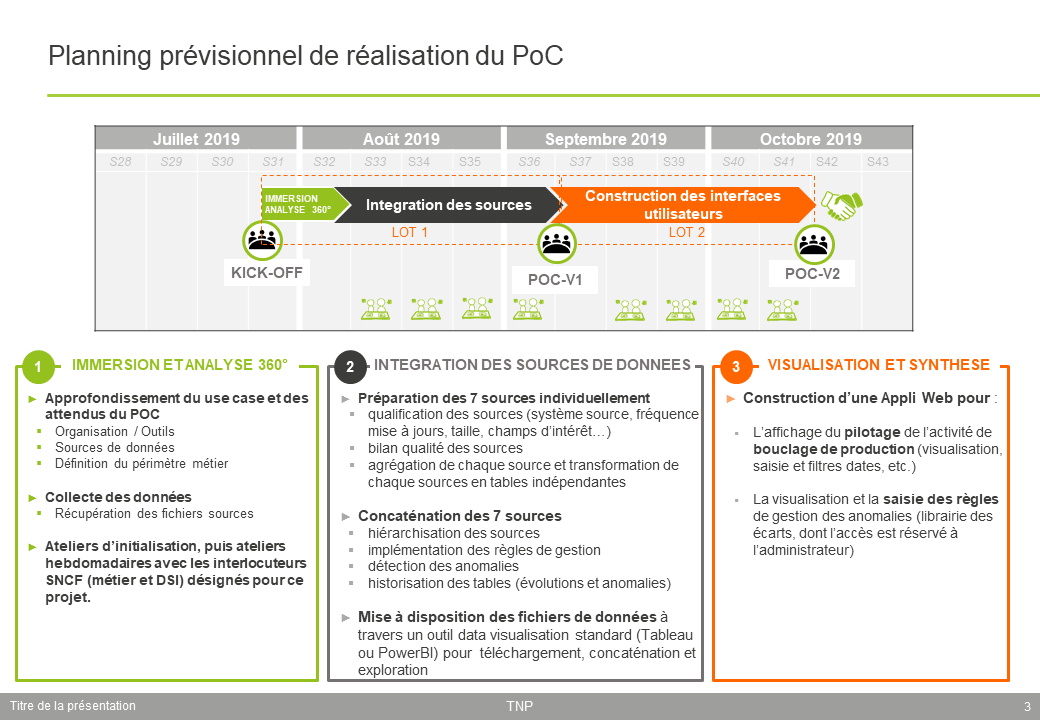
\includegraphics[width=1\linewidth]{img/planning-juillet-octobre-2019.png}
    \caption{Planning de la proposition de réalisation d'un POC}
\end{figure}

Grâce au \gls{poc}, on pourra valider la capacité à rendre la solution automatisable et industrialisable afin d'en faire le nouvel outil de partage et de communication entre les acteurs de la chaîne.


\paragraph{Immersion et analyse (juillet -- août)}

Tout d'abord une période d'\og immersion et d'analyse \fg a été mise en place pour permettre à l'équipe de \tnp de mieux comprendre l'état actuel de l'outil et sa mise en place pratique.\\
En effet, le \gls{poc} devra reproduire de manière automatisée la collecte et le traitement des données des différentes sources d'information de la \sncf.\\ L'équipe en profitera également pour poser toutes ses questions au
\gls{dsi}\footnote{\glsdesc{dsi}.}
et à l'équipe métier utilisant l'outil dans la pratique.


Une fois cette période passée, des réunions hebdomadaires ont été organisées avec le client pour obtenir ses retours et lui poser des questions si besoin sur certaines zones d'ombre.

\paragraph{Intégration des sources de données (août -- septembre)}

L'équipe data science de la \df a travaillé pendant un mois sur les traitements de données.

Les données de la \sncf sont dispersées dans presque une dizaine de sources. Les data science ont alors du préparer les données de chaque source afin d'en comprendre le fonctionnement, et l'information apportée par chacune.

Une fois ces sources préparées, il a fallu les agréger en une seule source complète et synthétique afin de les exposer nettoyées et traitées dans une base de données accessible avec des outils de visualisation de données comme PowerBI de Microsoft par exemple.

\paragraph{Visualisation et synthèse (septembre -- octobre)}

Les lot 1 et 2 n'ont pas pu être effectués en parallèle. Sans une idée de la structure et de la nature des données exposées par l'équipe data science, il aurait été difficile de commencer la création d'interfaces.

De plus, l'équipe \gls{ux}\footnote{\glsdesc{ux}} dirigée par \stefan a pu se servir du mois d'août pour recueillir le besoin métier du client et préparer des maquettes.


\begin{figure}[H]
    \centering
    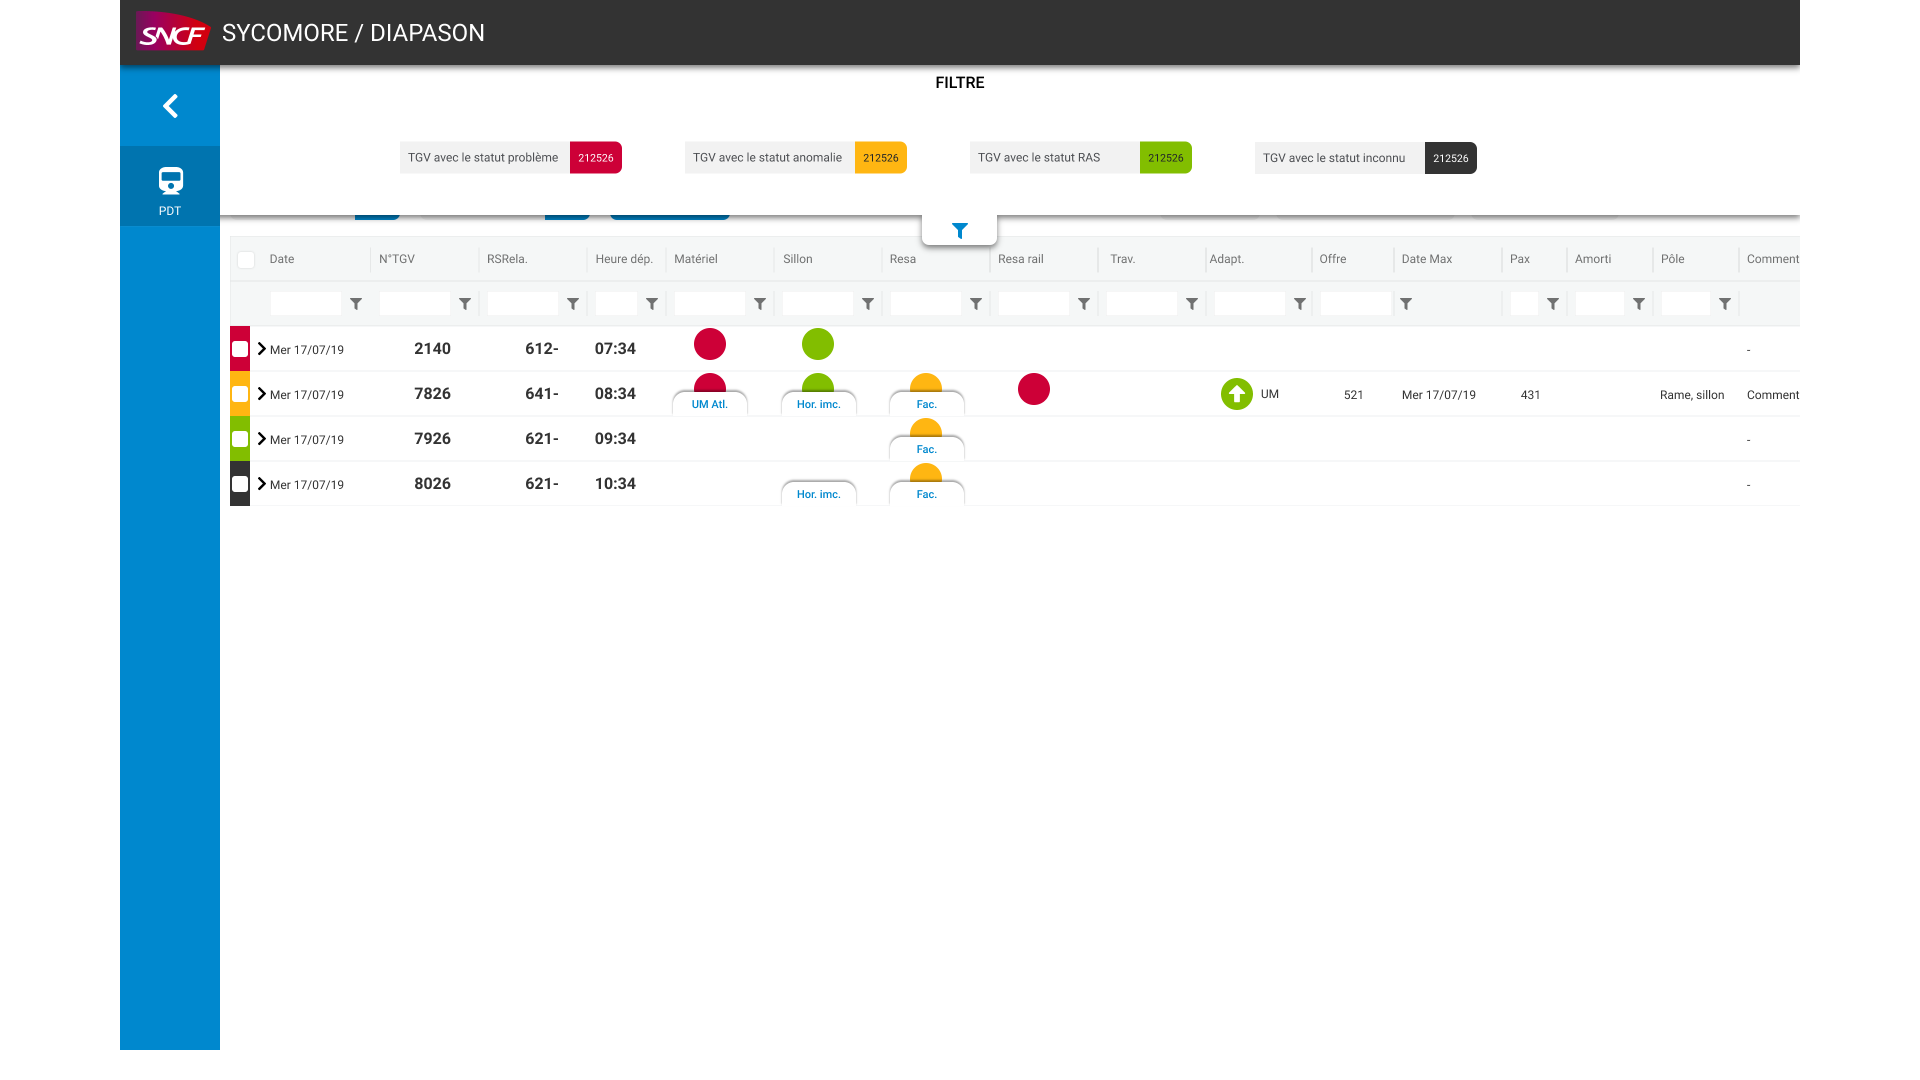
\includegraphics[width=1\linewidth]{img/maquette_home_page.png}
    \caption{Maquette de l'écran de visualisation des données synthétisées}
\end{figure}

Une fois les données rendues accessibles par les data science, et la maquette des \gls{ux} créée, l'équipe de développement a pu commencer la création de l'interface web.

L'objectif de l'interface était de présenter l'état de tous les trains sur une période donnée, avec des filtres pour accéder facilement à la donnée recherchée.\\
De plus, les équipes de la \sncf utilisent un jeu de règles pour la gestion des anomalies. Ils possèdent une bibliothèque des écarts -- appelée \og librairie des écarts, ou lib-écarts -- leur permettant d'assigner automatiquement un statut à un train en fonction des informations le concernant dans les différentes sources.


Ces règles permettent de classer automatiquement les trains en 3 états :

\begin{itemize}
    \item Rien à signaler (en vert sur la maquette)
    \item Situation anormale, mais traitée (en orange sur la maquette)
    \item Problème sur le train. Au moins un des acteurs de la chaîne nécessite une action (en rouge sur la maquette)
\end{itemize}

En plus de cette vue, l'administrateur doit avoir accès à un écran spécifique lui permettant de gérer ces règles -- ajout, suppression, modification.

En septembre 2019, l'équipe de développeurs était constituée de 4 développeurs : 2 \gls{front-end} et 2 \gls{full-stack}.

L'équipe des \gls{ux} -- composée de \stefan et d'un alternant sous sa tutelle -- avait une bonne compréhension du besoin client grâce à leur travail.

Ce dernier nécessitait de bien comprendre les usages métiers, et \stefan était très souvent présent aux réunions hebdomadaires. Ils étaient donc d'une précieuse aide pour aider les développeurs à comprendre le réel besoin métier derrière ces écrans.

Évidemment, \damien était aussi là pour apporter des clarifications et explications.

% , un consultant senior spécialisé en UX qui travaille pour la \df pendant ses temps d'inter-staffing\footnote{TODO}.

La partie \gls{front-end} consitait à reproduire les maquettes en y ajoutant les fonctionnalités de filtres, et l'écran de gestion des règles \og lib-écarts \fg.


Les développeurs \gls{full-stack} se sont chargé de créer la connexion entre les données récoltées par les data science et les renvoyer à l'interface en y ajoutant toutes les fonctions de filtre.

La gestion des règles lib-écarts devait également être gérée côté serveur pour envoyer la liste des règles à l'interface, et répercuter les changements lors des modifications.


De plus, un système de connexion et de gestion des utilisateurs a du être mis en place afin d'afficher les informations pertinentes pour la personne connectée.

En effet, l'administrateur doit, par exemple, avoir accès à l'écran de gestion des règles. Aussi, pour ne pas afficher des données inutiles, chaque axe ne  voit que les trains qui l'intéressent. Un filtre est alors appliqué par défaut à chaque utilisateur selon son axe.\\
Ainsi, la direction de l'axe Sud-Est n'a que faire de voir les trains de l'axe Atlantique.


En parallèle de la création de ces briques fonctionnelles, l'infrastructure cloud a été mise en place pour héberger l'applicatif créé.\\
Grâce à cela, la \df pouvait faire des démonstrations au client chaque semaine sans avoir besoin de tout installer sur son ordinateur. À terme, la \sncf avait aussi besoin d'un accès à l'applicatif pour effectuer sa recette fonctionnelle.

\subsubsection{Réalisation d'un MVP (décembre 2019 à mars 2020)}

Avec les grèves de fin d'année 2019, la première phase du projet a pris du retard. La deuxième phase a donc commencé en décembre 2019.

\begin{figure}[H]
    \centering
    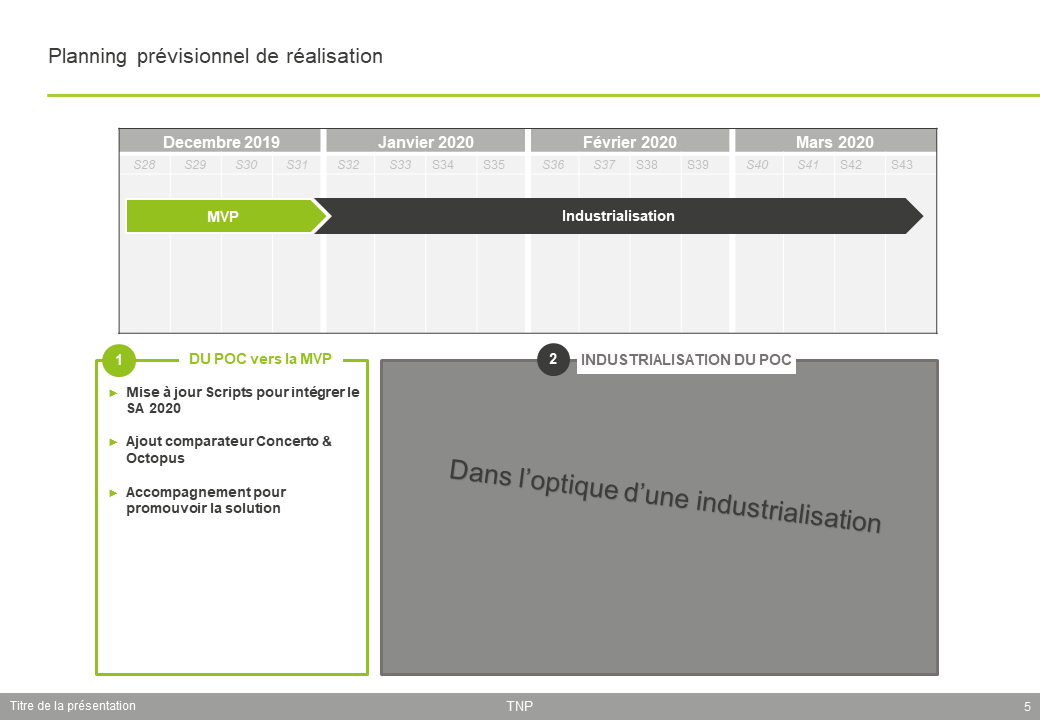
\includegraphics[width=1\linewidth]{img/planning-decembre-mars-2020-MVP.png}
    \caption{Planning de la proposition de réalisation d’un MVP}
\end{figure}

Cette étape du projet se focalise sur la conception d'un 
\gls{mvp}\footnote{\glsdesc{mvp}}
basé sur le \gls{poc} de l'étape précédente. Il est surtout question de faire évoluer le \gls{poc} vers une application plus fiable, à jour avec les nouvelles données de 2020 et ajouter une fonctionnalité de comparateur au projet.

Tous les 3 mois environ, les équipes de la \sncf produisent un nouveau document de synthèse pour leur bouclage de production avec de nouvelles données. La branche data science doit alors souvent adapter ses traitements aux changements de format de données, et également comprendre les potentiels nouveaux éléments dans les sources.

Pour l'équipe de développement, le \gls{mvp} consistait essentiellement à :

\begin{itemize}
    \item mettre à jour la vue synthétique avec les nouvelles données
    \item créer une page de comparateur entre deux sources
    \item corriger l'interface de gestion des règles lib-écarts.
    \item préparer l'écran d'import des mises à jour des données
\end{itemize}

Le comparateur entre la source Concerto et Octopus permet de... DEMANDER à DAMIEN.

Les règles de gestion lib-écarts ont été plus difficiles à gérer que prévu. En effet, l'utilisation et la création de ces règles a mal été compris et nous avons perdu du temps à essayer de comprendre leur fonctionnement.

En décembre, un 3ème développeur \textit{full-stack}\footnote{TODO} a rejoint l'équipe de la \df. Il s'est occupé de l'écran d'import des nouvelles données. Cet écran n'était pas compris dans ce lot, mais \damien savait que ce serait la prochaine étape demandée par le client. La page d'import permettra à terme aux utilisateurs de chez \sncf de téléverser les données sur l'application web pour lancer automatiquement les traitements et mettre à jour la vue synthétique.

% \subsubsection{Suite, industrialisation, problemes?}
% Hello world. Covid. Greves. Blocage SNCF.

% Enfin, une phase dite d'industrialisation...

